\documentclass{beamer}
\setbeamertemplate{navigation symbols}{}
\usepackage{beamerthemeshadow}
\usepackage{amsmath}
\usepackage{float}
\usepackage{graphicx}
\usepackage{listings}
\usepackage{caption}
\usepackage{subcaption}
\usepackage[T1]{fontenc}
\usepackage[brazilian]{babel}
\usepackage{geometry}
\usepackage{lmodern}
\begin{document}

\title{title}
\author{author}
\date{february 2015}
\begin{frame}
\titlepage
\end{frame}
\maketitle


\begin{frame}\frametitle{Table of Contents}
\tableofcontents
\end{center}

\section{Haskell}

\begin{frame}\frametitle{The frame ith name}
\lstset{language=haskell}
\begin{lstlisting}[frame=single]
main = do
  as <- getArgs
  return as
\end{lstlisting} 

 \lstset{language=C}
\begin{lstlisting}[frame=none]
int main (args* char[]){
   return c + 3;
}
\end{lstlisting}
\end{frame}

\begin{frame}\frametitle{Frame with color}
{\color{yellow}This text is yellow} 
 {\color{red}This is red!} 
 {\color{green}greeeeeeeeeeeeeeeeeen} 

 \begin{center}\centering{\tt asdasdasdasdasda
sdfasdfa
sdfasdfa
sdfasdfasdf
asdfasfdasdf hey hey}\end{center}
\end{frame}

\begin{frame}\frametitle{another frame}
\begin{equation}\label{a^5}
= b^5 + c^5 + \int^{\inf}_{0}dx^5
\end{equation} 

$$\vec{a}^5 + \mathbf{a} = \sin{3423414}$$

 \begin{figure}[H]
\centering
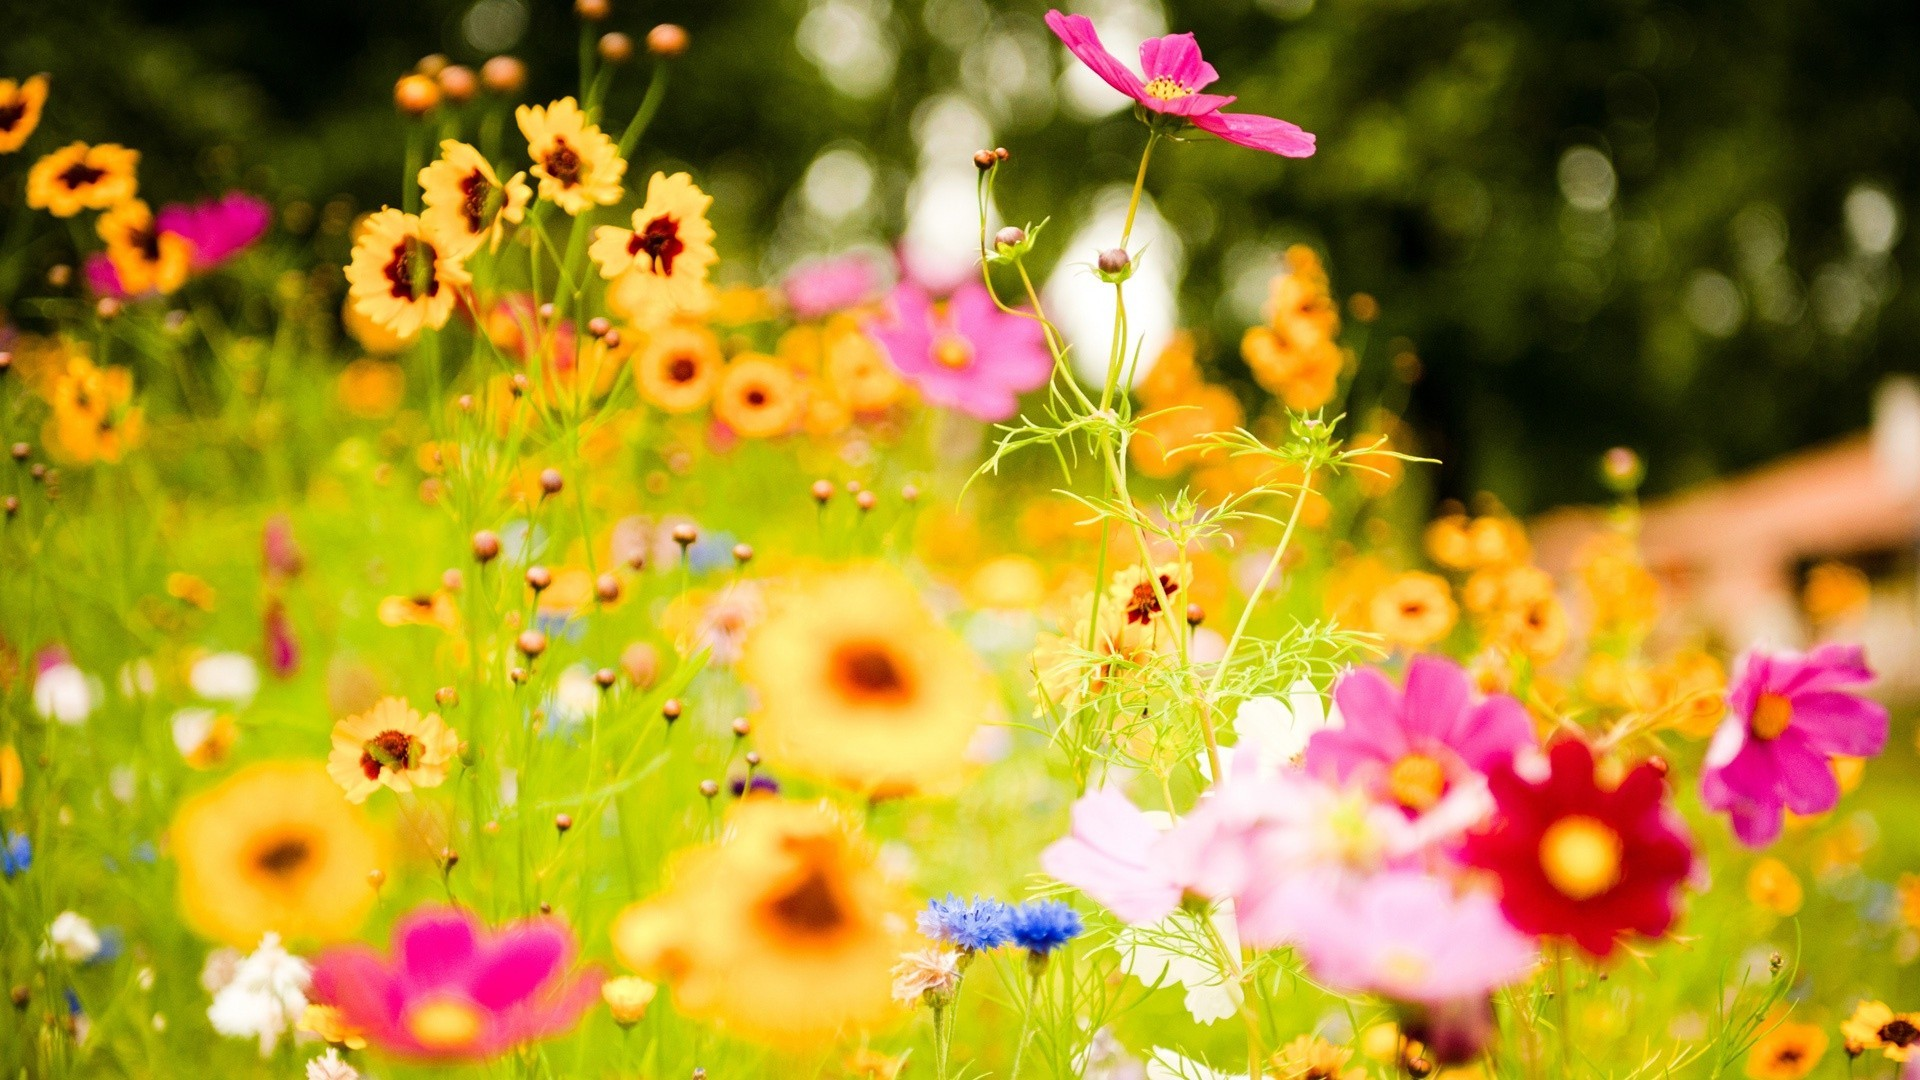
\includegraphics[width=10cm]{../../External/Images/flowers}
\caption{flowers}
\end{figure}
 

 {\tt Richard Feynman} 

 \begin{enumerate}
\item isso ai
\item asdasdasd
\item asda
sdasd
\item asdasdasdsa
\item thats is
\item \lstset{language=haskell}
\begin{lstlisting}[frame=none]
main = do...
\end{lstlisting}
\end{enumerate}
\end{frame}

\begin{frame}\frametitle{last frame}
{\tt asdasdasdasdasda
sdfasdfa
sdfasdfa
sdfasdfasdf
asdfasfdasdf hey hey}
\end{frame}

\end{document}